\begin{frame}{Hypothèses formulées}
	\begin{enumerate}
		\item 	Le texte comme point d'entrée pour étudier les tendances de la circulation des idées à l'aide des caractéristiques structurelles.
			\begin{flushright}
			\small
			\parencite[p.~2]{milia2023}
		\end{flushright}
		
		\item Certains termes médicaux associés à Charcot ont été repris de manière significative dans les écrits de son réseau scientifique.
		
		\item Chronologie d'une locution : indice de croissance de l'impact.
			\begin{figure}[h] % Use [H] to force the figure to stay in place
			\begin{itemize}
				\item évolution de la fréquence des termes au sein des deux corpus\footnote{\url{https://obtic.huma-num.fr/obvie/charcot/?view=corpus}}
				\item ex. : convergence entre des termes : fin \textsc{XIX}\ieme{}, début \textsc{XX}\ieme{} s.
				%		\begin{itemize}
					%				\item \textit{ppm} : nombre d’occurrences par million de mots 
					%		\end{itemize}
			\end{itemize}
			\centering
			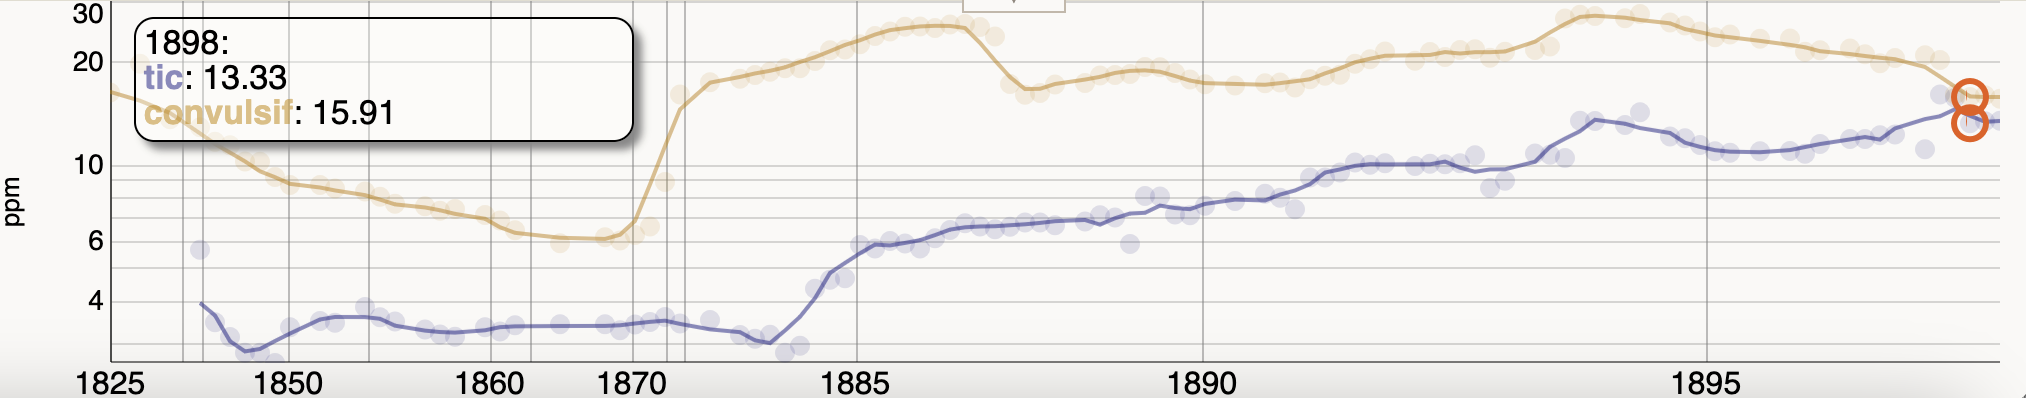
\includegraphics[width=\linewidth]{pic/tics_convulsifs.png}
			\caption{Chronologie de la fréquence du terme \textit{tic convulsif}.}
			\label{fig:ling_out_TAL}
		\end{figure}
	\end{enumerate}

	
%	\begin{block}{\begin{enumerate}
%
%		\end{enumerate}}
%	\end{block}
\end{frame}

%\begin{frame}{Chronologie d'une locution : indice de croissance de l'impact ?}
%	\begin{figure}[h] % Use [H] to force the figure to stay in place
%		\begin{itemize}
%			\item évolution de la fréquence des termes au sein des deux corpus\footnote{\url{https://obtic.huma-num.fr/obvie/charcot/?view=corpus}}
%			\item convergence entre des termes : fin \textsc{XIX}\ieme{}, début \textsc{XX}\ieme{} s.
%			%		\begin{itemize}
%				%				\item \textit{ppm} : nombre d’occurrences par million de mots 
%				%		\end{itemize}
%		\end{itemize}
%		\centering
%		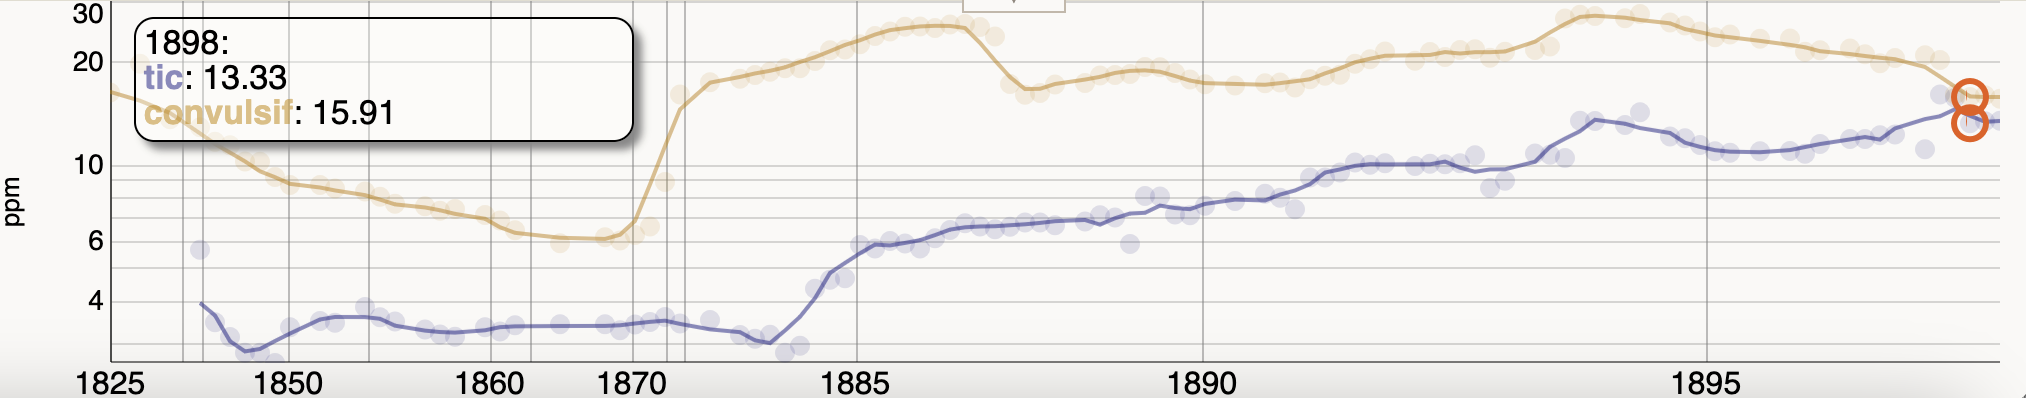
\includegraphics[width=\linewidth]{pic/tics_convulsifs.png}
%		\caption{Chronologie de la fréquence du terme \textit{tic convulsif}.}
%		\label{fig:ling_out_TAL}
%	\end{figure}
%	
%	\begin{figure}[h]
%		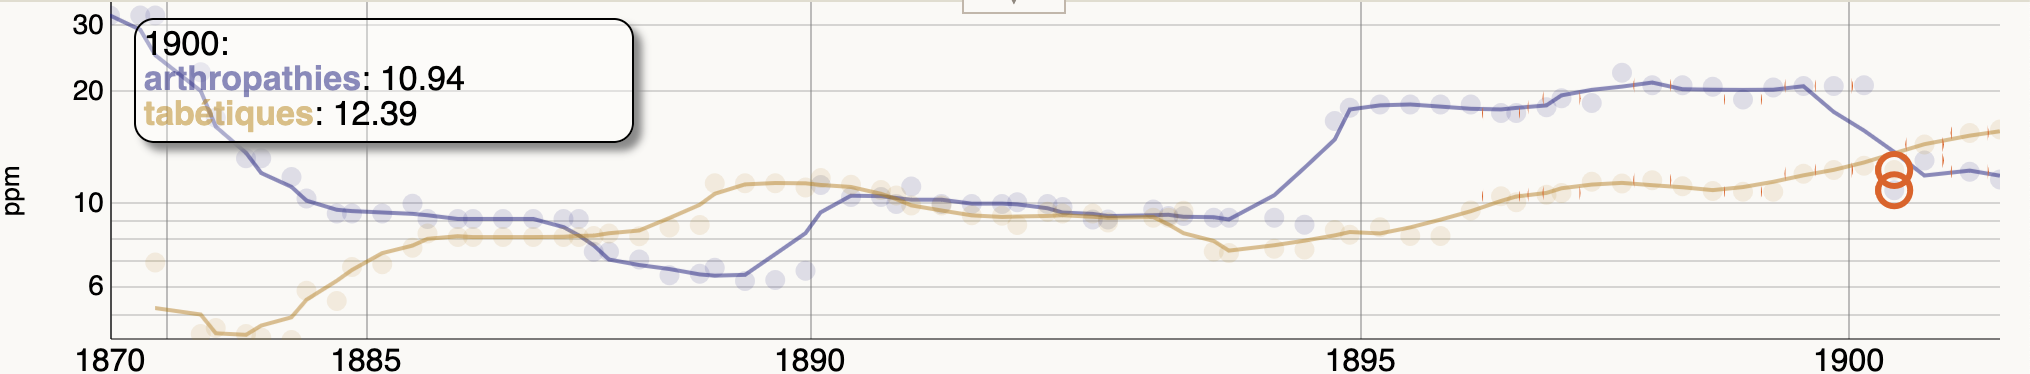
\includegraphics[width=\linewidth]{pic/arthropathies_tabetiques.png}
%		\caption{Chronologie de la fréquence du terme \textit{arthropathies tabétiques}.}
%		\label{fig:ling_out_TAL}
%	\end{figure}
%\end{frame}